% pour générer un pdf: faire
% pdflatex exemple.tex
\documentclass{article}

%% Paquets LateX utiles

\usepackage[utf8]{inputenc} 		% encodage des caractères utilisés (pour les caractères accentués) 
% pour les accents, on peut soit préciser l'encodage et utiliser des caractères accentués, soit utiliser é pour un e accent aigu, \`e pour un e accent grave, etc...
%\usepackage[latin1]{inputenc} 		% autre encodage
\usepackage[french]{babel}		% pour une mise en forme "francaise"
\usepackage{amsmath,amssymb,amsthm}	% pour les maths
\usepackage{graphicx}			% pour inclure des graphiques
\usepackage{hyperref}			% si vous souhaitez que les references soient des hyperliens
\usepackage{color}			% pour ajouter des couleurs dans vos textes
\usepackage{parskip}


% Définitions de macro
\def \dd {\mathrm{d}}

\title{Barrages et Risques d'Inondation}
\author{Zian Chen \& Ruikai Chen}	

\begin{document}
\maketitle						% Génère le titre

%\tableofcontents					% si on veut une table des matieres
%\listoffigures						% si on veut la liste des figures
%\listoftables						% si on veut la liste des tableaux
\section{Introduction}
Un barrage est un ouvrage artificiel ou naturel, établi en travers du lit
d'un cours d'eau, retenant ou pouvant retenir de l'eau. Les barrages ont plusieurs fonctions, par exemple : la régulation de cours d'eau; l'irrigation des cultures; la lutte contre les incendies, etc. La rareté des accidents est le résultat d'efforts attentifs depuis un siècle.

Dans ce projet, nous allons étudier les risques d'inondation en utilisant des méthodes probabilistes. Nous allons modéliser les volumes des lacs, et étudier les risques d'inondation avec plusieurs algorithmes de simulation. Plus précisement, nous allons trouver les seuils de volumes pour que les barrages soient en sécurité avec une probabilité très élevée (par exemple, 99.9999\%). Dans la deuxième section, nous allons modéliser les volumes des lacs en compte de l'apport de l'eau et la lâchers d'eau. Dans la troisième section, nous étudions les risques d'inondation avec des algorithmes différentes et considérons quelques situations différentes. Dans la quatrième section, nous présentons les résultats de simulation numérique.
\section{Modélisation}
Nous supposons que, dans une région montagneuse, deux vallées
sont occupées par deux lacs artificiels créés par deux barrages $B_1$ et $B_2$. Nous allons modéliser les volumes des lacs $(X_t^i)$ au cours du temps $t$ en compte de l'apport de l'eau et la lâchers d'eau. Plus précisement, nous avons
\begin{equation}\label{eq_X}
  X_t^i = x_0^i + A_t^i - \int_0^t r_iX_s^i  ds,
\end{equation}
où $x_0^i$ est le volume initial, $A_t^i$ est le volume total de pluie au temps $t$, $r_i$ est le taux de lâchers d'eau du lac $i$.
\paragraph{Modélisation de l'apport de l'eau} Nous supposons que l'apport d'eau $A^i_t$ est essentiellement déterminé par des chutes de pluie intenses
et de courte durée. Autrement dit $A_t^i$ est un processus de Poisson composé,
\[A_t^i = \sum_{n=1}^{N_t^i} U_n^i,\]
où $N_t^i$ est un processus de Poisson de taux $\lambda_i$ qui décrit l'arrivée de pluie, et $U_n^i$ suit une combinaison exponentielle de paramètres $\delta_1$ et $\delta_2$ qui modéliser séparément des pluies de grande et petite intensité :
\[\nu(u) = b\delta_1\exp(-\delta_1 u)\mathbf{1}_{u\geq 0} + (1-b)\delta_2\exp(-\delta_2 u)\mathbf{1}_{u\geq 0}.\]
Nous choisissons $\delta_2/\delta_1$ de l'ordre de 10 et $\delta_2 = 0.7$.
\paragraph{Calculs du volume d'eau dans le lac} Si nous représentons le processus de Poisson composé par une série de sauts, i.e.
\[N_t^i = \begin{cases}0&\textrm{pour $t\in [0, T_1[$,}\\
  1&\textrm{pour $t\in [T_1, T_2[$,}\\
  2&\textrm{pour $t\in [T_2, T_3[$,}\\
  \vdots &\quad\vdots\end{cases}\]

Alors la solution de Eq. \ref{eq_X} est donnée par
\[X_t^i = \exp(-r_i t)\left(\int_0^t \exp(-r_i s)\dd A_s^i + x_0^i\right),\]
où \[\dd A_s^i=\begin{cases} U_s^i\delta_s &\text{si } s\in \{T_1,T_2,\cdots\}\\
  0&\text{sinon}\end{cases}\] 
au sens de distribution, autrement dit
\[X_t^i = \begin{cases}x_0^i\exp(-r_i t)&\textrm{pour $t\in [0, T_1[$,}\\
  \exp(-r_i t)(x_0^i+\exp(r_i T_1)U_1^1)&\textrm{pour $t\in [T_1, T_2[$,}\\
  \exp(-r_i t)(x_0^1+\exp(r_i T_1)U_1^1+\exp(r_i T_2)U_2^i)&\textrm{pour $t\in [T_2, T_3[$,}\\
  \vdots &\quad\vdots\end{cases}\]

\begin{figure}[t]
  \centering
  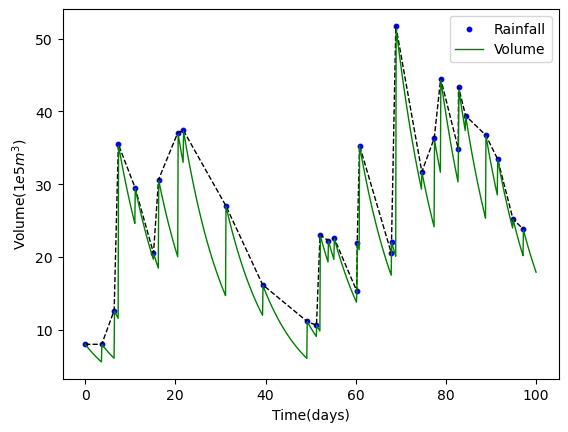
\includegraphics[width=0.7\textwidth]{rainfall.png}
  \caption{Une simulation du volume d'eau pour $\lambda=0.3$, $b=0.5$, $\delta_1=0.07$, $\delta_2=0.7$, $r_i=0.1$, $x_0^i=8$ dans les unités de <<jour>> et <<$10^5m^3$>>. La courbe verte représente l'évolution du volume au cours du temps. Les points bleue représente les volumes d'eau après chaque pluie.}
  \label{v_e}
\end{figure}

Une illustration des évolutions de volume d'eau est donnée dans le figure \ref{v_e}. Nous remarquons que nous pouvons obtenir deux types des données : les volumes d'eau après chaque pluie, qui a la même longeur que les chutes de pluie, et les volumes d'eau au cours de temps. En général, le premier type de donnée est suffisant, car nous considérons principalement le rique d'inondation.

\section{Risque d'inondation}
Dans cette section, nous allons introduire de différentes approches pour simuler le rique d'inondation. Pour un premier temps, nous considérons le cas d'un seul barrage. Et puis nous prenons en compte des intersections de deux barrages.
\subsection{Le cas d'un seul barrage}
Quand il y a un seul barrage qui est présent, nous utilisons les notations sans indice $i$ comme $X_t$ et $A_t$. et nous formulons le problème de rique d'inondation comme suit : nous voulons trouver le seuil $x^\ast$ (soit pour un certain $T$, on prend $X=X_T$, soit pour le volume maximum dans $[0,T]$, on prend $X=\max_{0\le s\le T}X_s$) tel que
\[\mathbb{P}(X>x^\ast)\leq \alpha.\]
\paragraph{Monte-Carlo naïf} La méthode de Monte-Carlo naïf pour trouver un quantile $1-\alpha$ est de simuler $N$ trajectoires de $X$, notons $(X_i)$ et de prendre le quantile empirique. Nous rappelons que le quantile empirique est donné par
\[\hat{q}_{1-\alpha} = \inf\{x\in \mathbb{R}:\hat{F}_N(x)\geq 1-\alpha\},\]
où $\hat{F}_N$ est la fonction de répartition empirique. 
\[ \hat{F}_N(x) = \frac{1}{N}\sum_{i=1}^N \mathbf{1}_{X_i\leq x}.\]
Si nous trions les valeurs de $X_i$ comme $X_{(1,N)}\leq X_{(2,N)}\leq \cdots \leq X_{(N<N)}$, alors nous avons
\[\hat{q}_{1-\alpha} = X_{(\lceil N(1-\alpha)\rceil,N)}.\]
Cet algorithme est réalisé comme méthode $\texttt{get\_critical\_level}$ dans la classe $\texttt{naive\_MonteCarlo}$.
\paragraph{Importance Sampling (Esscher)}
\paragraph{Algorithme de la dernière particule}

L'idée de l'algorithme de la dernière particule est de renouveler la valeur minimale d'une suite de $X$ selon la loi de $(X|X>L)$ où $L=\min(X_i)$. 

Précisément, on simule d'abord une suite, notons $(X_i)_{1\leq i\leq n}$, selon la loi de $X$. On note le minimun temporaire $L=\min_{1\leq i\leq n}(X_i)$, et on remet à jour ces $X_i$ égaux à $L$ par un échantillon indépendant selon la loi de $(X|X>L)$. En répétant ce processus $\displaystyle \left\lceil\frac{\log \alpha}{\log(1-1/n)}\right\rceil$ fois, le minimum final $L$ est le seuil dont on a besoin.

Il nous reste à obtenir un échatillon selon la loi de $(X|X>L)$. Rappelons que $X_t$ est obtenu du processus de Poisson composé $A_t$, d'où il suffit de mettre à jour $A_t$ correspondant. L'idée est à partir d'une autre particule, on fait $M$ itérations pour que ce soit presque indépendent de celle originale. Pour ce faire, on utilise l'algorithme de coloriage pour renouveler $N_t$ et pour des $U_i$, on obtient une combinaison des valeurs originales et des échantillons indépendants si le $i$-ième saut est gradé, où la proportion $q$ sera considérée dans la partie numérique.

On a deux méthodes dans la programmation, la méthode $\texttt{get\_new\_rainfall}$ et l'autre $\texttt{get\_critical\_level\_and\_distribution}$ dans la classe $\texttt{last\_particle}$.

\section{Simulation numérique} 
\paragraph{Paramètres physiques} On met l'unité de temps comme $1$ an et l'unité de volume comme $10^5m^3$. On a que $r^i=1$ et $T=1$. On suppose qu'il pleut $\lambda=70$ fois par an. On fixe en plus $\delta_1=0.07$ et $\delta_2=0.7$, où son unité est $(10^5m^3)^{-1}$ et l'inverse de $\delta_i$ montre le volume moyen d'une seule pluie. Le quantile $\alpha$ considéré est $10^{-6}$, et on prend la proportion $b=0.1$, i.e. seule une sur dix est une grande pluie.

Maintenant on va considérer la valeur de $x_0$, le volume initial. On veut que $x_0$ soit <<l'état stationnaire>> pour que ce soit compatible avec le processus physique, i.e. le flux d'eau entrant et sortant est presque équilibré pendant assez longtemps. Dans la pratique, on simule $5000$ fois $X_{100}$ et puis calcule le moyen, cela nous donne $x_0=190$.

Cette idée peut aussi être réalisée par un calcul théorique. Pour un petit temps $\Delta t$, le flux sortant est $-(r_1 x_0)\Delta t$ alors que le flux entrant est $\mathbb E[\nu](\lambda_1\Delta t)$. Pour que $x_0$ soit l'état stationnaire, on a forcément que  $-r_1x_0+\lambda_1{\mathbb E[\nu]}=0$, d'où
\[x_0=\frac{\lambda_1}{r_1}\left(\frac{b}{\delta_1}+\frac{1-b}{\delta_2}\right)=190.\]
\end{document}


